%---------- Inleiding ---------------------------------------------------------

\section{Introductie}
\label{sec:introductie}
Vandaag de dag kent sport een prominente rol bij vele Vlamingen, dat kunnen we duidelijk aflezen uit statistieken van~\textcite{StatistiekVlaanderen2023}.
Hoewel sporten centraal staat voor gemiddeld \'e\'en op de vijf Vlamingen, kampt de sportsector met een sterk trainerstekort. \autocite{SportVlaanderen2023}
Met de toenemende groei van de artifici\"ele intelligentiesector ontstaat de mogelijkheid voor bijkomende hulpmiddelen om de werkdruk van trainers te verlichten.
Hierbij kunnen machine learning en objectdetectie bijdragen tot het personaliseren van een trainingsschema voor een gebruiker.
Met de opkomst van steeds slimmere AI-tools kan de drempel om te starten bovendien verlaagd worden voor startende fitnessliefhebbers.

Door de explosie aan aandacht naar artifici\"ele intelligentie en objectdetectie onstaan er mogelijkheden om nauwkeuriger resultaten te bieden aan een kleinere technologische barri\`ere.
De vraag ontstaat dan ook of fitnessclubs deze technologie\"en kunnen toepassen om het makkelijker te maken voor startende sporters en de kans op het afhaken van trainers op de lange termijn te verlagen.
Deze thesis probeert een ondersteunde oplossing te zoeken op een gebruiksvriendelijke en rendabele manier.
Zo kunnen gebruikers een fitnessschema voorgesteld krijgen door het simpelweg inscannen van de gewenste fitnessapparatuur met een mobiele telefoon.
Met machine learning kan deze apparatuur vervolgens gedetecteerd worden en kan de beginnende sporter beginnen aan zijn work-out.
Trainers kunnen makkelijk hier op voortbouwen en het trainingsschema aanvullen en hebben van in het begin een zicht op de beschikbare apparatuur.

%---------- Stand van zaken ---------------------------------------------------

\section{Literatuurstudie}
\label{sec:state-of-the-art}

\subsection{Artificiële intelligentie}
\label{subsec:artificiele-intelligentie}
Hedendaagse artifici\"ele algemene intelligenties komen voornamelijk voort uit vooraf getrainde taalmodellen.
Aan de hand van natuurlijke taalverwerking (NLP) krijgt de intelligentie een inzicht in wat ervan verwacht en hoe het hoort te reageren op interactie van de gebruiker.
De verwerkte gegevens bestaan uit een brede dekking aan informatie afkomstig van bronnen die kunnen vari\"eren van nieuws artikelen tot taalexamens, aldus~\textcite{Liu2019}.

2022 kende een explosie in de waar te nemen mogelijkheden van kunstmatige intelligentie gestuurd door deze natuurlijke taalverwerkingsmodellen.
OpenAI bracht haar derde generatie Generative Pre-trained Transformer (GPT) model uit en markeerde hiermee de nieuwe standaard van deep learning modellen.
Het naar het model genoemde GPT-3 platform toonde belovende eerste resultaten bij het experimenteren rond het literaire aspect~\autocite{Elkins2020}, zo kon het model kwaliteitsvollere filosofische essays genereren dan bestaande geschreven essays.
Ondanks deze resultaten bleek het model volgens~\textcite{Floridi2020} geen dieper begrip te kennen van het gegenereerde resultaat.

Slechts een jaar later, in maart 2023, kwam de volgende generatie uit van OpenAI's Generative Pre-trained Transformer (GPT) model.
Het GPT-4 platform is in elk opzicht beter dan het GPT-3 platform volgens de resultaten van~\textcite{Katz2023}, en in een opmerkelijk opzicht, ook beter dan de gemiddelde persoon in vijf van de zeven deelgebieden in het Multistate Essay Exam (MEE), een gedeeltelijk toelatingsexamen om rechter te worden in de Verenigde Staten.

\subsection{De technologische vooruitgang van objectdetectie in de cloud}
\label{subsec:effect-objectdetectie-cloud}
Met de komst van het GPT-4 platform ontstond de mogelijkheid om naast tekst ook bestanden, waaronder foto's, in te voeren.
Als reactie op het succes van OpenAI's (Chat)GPT kwam Google met haar eigen AI-platform, genaamd Bard (nu Gemini).
Gemini kent nu ook al een integratie in Google's Cloud Vertex AI, wat de nauwkeurigheid en bruikbaarheid van object detectie in foto's sterk bevordert.~\autocite{GoogleCloud2024}
Hiermee wordt het steeds interessanter om gebruik te maken van Google Cloud om gebruik te maken van machine learning.

\subsection{Lokale machine learning}
\label{subsec:benefits-hmd}
Echter zijn er ook nadelen bij clouddiensten zoals Google Cloud: niet elke organisatie is groot genoeg om het gebruik van clouddiensten te kunnen verantwoorden.
Een alternatief hiervoor is het lokaal draaien van machine learning.
Mogelijke opties hiervoor zijn PyTorch en TensorFlow.
Hoewel deze tools ongetwijfeld sneller zullen draaien op servers in de cloud, is het ook mogelijk om hier gebruik van te maken op een lokale computer.
Een moderne videokaart (hetzij de workstation Quadro-lijn of de consumenten-gerichte GeForce-lijn) van NVidia, of zelfs moderne videokaarten van AMD via het ROCm platform.~\autocite{AMD2024}
De nauwkeurigheid en snelheid zal lager liggen dan datasets gegenereerd door middel van cloudservices, maar aan een fractie van de kost.
Het vergelijken van een cloudoplossing met een lokale machine tijdens de proof-of-concept fase van deze thesis kan hierbij interessant zijn.

%---------- Methodologie ------------------------------------------------------
\section{Methodologie}
\label{sec:methodologie}
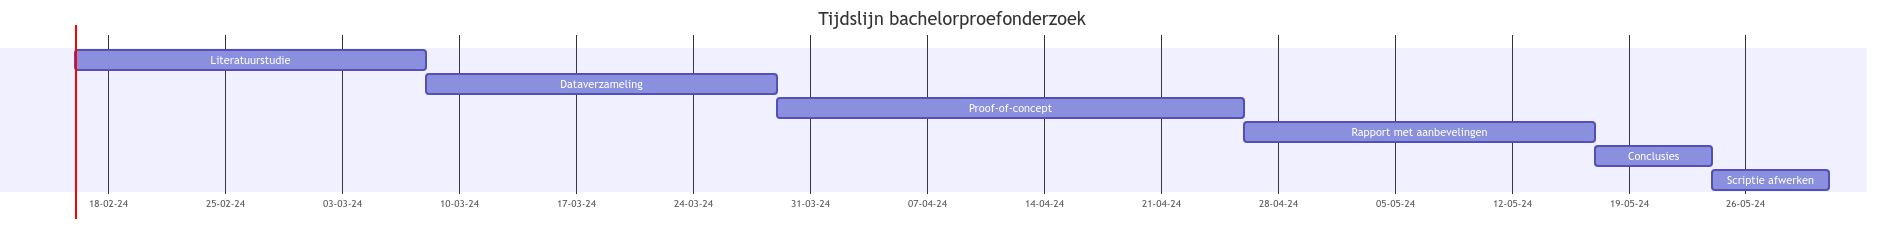
\includegraphics[width=1\textwidth]{images/ganttChart}

\subsection{Voorafgaande literatuurstudie}
\label{subsec:literature-study}
In de eerste fase vindt zich een voorafgaande literatuurstudie over het onderwerp plaats. % 3 weken
Het praktische doel hiervan is om een verdere inzicht te krijgen op de werking van machine learning en haar rol bij object detectie op foto's.
De nadruk ligt hierbij op de evolutie van deze werking en de verschillen tussen lokale machine learning applicaties en die van cloudproviders zoals Amazon en Google.
Tijdens deze fase komen de gelijkenissen en verschillen tussen de twee varianten aan bod om tijdens de derde fase te kunnen vergelijken aan de hand van een proof-of-concept.

\subsection{Dataverzameling}
\label{subsec:dataverzameling}
Vervolgens vindt er zich een requirements-analyse plaats om af te toetsen waar de focus moet liggen bij objectdetectie. % 3 weken
Gebruikers die een app gebruikmakend van deze tool wensen te gebruiken tijdens het sporten horen eender welke gerelateerde apparatuur in te kunnen scannen.
Om dit te realiseren moet de dataset getraind worden op gepaste en gevarieerde fitnessapparatuur in verschillende fitnessclubs.
Hiervoor wordt data in de vorm van foto's en beschrijvingen verzameld, gepaard met de gebruiksmogelijkheden en eventuele advies van trainers.
Dit wordt vervolgens gegoten in bruikbare datasets in de derde fase.
Ook zal hiermee de mogelijkheid ontstaan voor gebruikers om een gepersonaliseerd fitnessschema aan te bieden, deels vooropgesteld door trainers.

\subsection{Proof-of-concept}
\label{subsec:poc}
Gedurende de derde fase wordt een proof-of-concept applicatie gebouwd voor Android-apparaten. % 4 weken
Hiervoor worden er eerst datasets gegenereerd voor de objectdetectie functionaliteit.
Deze datasets zullen enerzijds gebruik kunnen maken van de machine learning capaciteiten van Google Cloud (Vertex AI) of anderzijds gegenereerd worden op een lokale computer gebruikmakend van het TensorFlow framework.
Hiermee kunnen we het verschil in kwaliteit testen om vervolgens de waarde van de platformen af te toetsen tegenover de kostprijs.
De proof-of-concept toetst de mogelijke antwoorden die tijdens de literatuurstudie aan bod kwamen op de requirements af.

\subsection{Rapport met aanbevelingen}
\label{subsec:result-of-poc}
Na het opzetten van de proof-of-concept komen enkele gebruikerstests aan bod. % 3 weken
Hierbij worden het gebruikspatroon, de tijdsduur en foutenpercentage van objectdetectie vastgelegd.
Een analyse van deze cijfers zal de bruikbaarheid van het gebruiken van objectdetectie en genereren van gepersonaliseerde trainingsschema's aantonen.
Daaropvolgend wordt een rapport met aanbevelingen opgesteld voor ontwikkelaars die soortgelijke functies willen implementeren.
Belangrijk hierbij is dat ontwikkelaars dit rapport kunnen gebruiken om te kunnen kiezen tussen een lokaal gegenereerde dataset of gebruikmakend van clouddiensten zoals Google Cloud.

%---------- Verwachte resultaten ----------------------------------------------
\section{Verwacht resultaten en conclusie}
\label{sec:verwacht-resultaten-en-conclusie}
Er wordt verwacht dat de resultaten uit de proof-of-concept zal leiden tot een bruikbare tool die de drempel tot het starten van sport verlagen.
Deze tool zal concreet de mogelijkheid bieden om fitness apparatuur in te scannen en detecteren door middel van machine learning.
Hiermee kunnen ontwikkelaars die werken voor fitnessketens snel aan de slag voor gepersonaliseerde applicaties.
De hypothese stelt dat de drempel om te starten in een fitnessclub zal verlaagd worden en dat coaches meer kunnen focussen op langetermijnschema's.
Aan de hand van het aanbevelingsrapport kunnen ontwikkelaars ervoor kiezen om gebruik te maken van Google Cloud voor nauwkeurigere oplossingen of voor een lokale machine voor een lagere kostprijs.